\documentclass[times, utf8, seminar, numeric]{fer}
\usepackage{booktabs}
 \usepackage{url}
 \usepackage{tikz}
 \usepackage{todonotes}
 \usepackage{minted}
 
 
 \usetikzlibrary{matrix}
 \usetikzlibrary{external}
 \tikzexternalize[prefix=build/]
 
 \setminted{fontsize=\small,baselinestretch=1,linenos,frame=lines}
 
 \renewcommand{\listingscaption}{Programski isječak}
 \renewcommand*{\thelisting}{\thechapter.\arabic{listing}}
 
 

\begin{document}

% Ukljuci literaturu u seminar
\nocite{*}

\title{Pronalazak najkraćeg puta algoritmom A*}

\author{Marko Lazarić}

\voditelj{Doc. dr. sc. Marko Čupić}

\maketitle

\tableofcontents

\chapter{Uvod}
Velik broj problema može se modelirati grafom u kojem vrhovi predstavljaju stanja, a bridovi prijelaze između tih stanja, takav graf se naziva prostor stanja \engl{state space}.
Rješavanje problema se onda svodi na pretraživanje prostora stanja, odnosno pronalazak najkraćeg puta između početnog stanja i stanja koje predstavlja rješenje problema.

% Problem pronalaska najkraćeg puta između dva vrha u grafu jedan je od najstarijih i najbolje istraženih problema u teoriji grafova. Rješenja tog problema imaju široku primjenu jer se velik broj situacija u pravom svijetu može modelirati kao grafovi, gdje vrhovi predstavljaju stanja, a bridovi prijelaze između tih stanja. Provedbom ovih algoritama minimizira se broj prijelaza, odnosno trošak za prijelaz od početnog do završnog stanja.

Zbog svoje široke primjenjivosti, osmišljeni su razni algoritmi za efikasno rješavanje tog problema. U ovom seminaru razmatrat će se prednosti i mane različitih algoritama za pronalazak najkraćeg puta između dva vrha u grafu, počevši od jednostavnijih naivnih algoritama,  do složenijih za implementaciju, ali efikasnijih informiranih algoritama s naglaskom na algoritam A* i njegovu primjenu na pronalazak najkraćeg puta u cjelobrojnoj rešetci. 

U svrhu jednostavne vizualizacije rada algoritama, koristit će se cjelobrojna rešetka u kojoj sivi kvadratići predstavljaju neprolazna polja, dok bijeli predstavljaju polja kroz koja se može proći. Moguće je kretati se u 4 osnovna smjera. "A" predstavlja početno stanje (vrh), a "B" završno. 

\begin{figure}[h]
	\centering
	
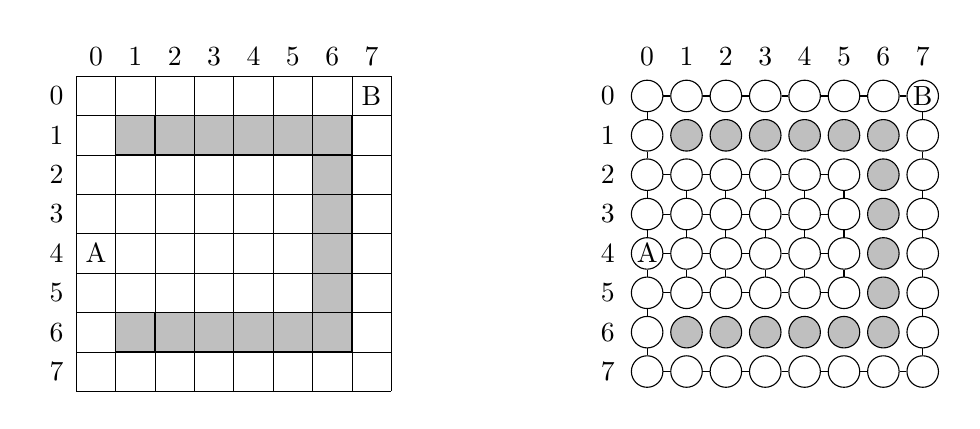
\begin{tikzpicture}
	\begin{scope}
		\begin{scope}[xshift=0.25cm, yshift=-0.25cm]
	\draw[step=0.5cm,black,very thin] (-2,-2) grid (2,2);
	
	\newcommand\fillSquare[2]{\filldraw[fill=lightgray] (#1 / 2,#2 / 2) rectangle (#1 / 2 + 0.5,#2 / 2 + 0.5)}
	
	
	\foreach \x in {-3,...,2}
	{
		\fillSquare{\x}{-3};
		\fillSquare{\x}{2};
		\fillSquare{2}{\x};
	}
\end{scope}

\matrix[matrix, matrix of nodes, nodes={anchor=center,inner sep=0pt,text width=.5cm,align=center,minimum height=.5cm}, nodes in empty cells]{
& 0 & 1 & 2 & 3 & 4 & 5 & 6 & 7 \\
 0 &   &   &   &   &   &   &   & B \\
	1 &   &   &   &   &   &   &   &   \\
	2 &   &   &   &   &   &   &   &   \\
	3 &   &   &   &   &   &   &   &   \\
	4 & A &   &   &   &   &   &   &   \\
	5 &   &   &   &   &   &   &   &   \\
	6 &   &   &   &   &   &   &   &   \\
	7 &   &   &   &   &   &   &   &   \\};
	\end{scope}
	
	\begin{scope}[xshift=7cm]
	    \matrix[matrix, matrix of nodes, nodes={anchor=center,inner sep=0pt,text width=.5cm,align=center,minimum height=.5cm}, nodes in empty cells]{
   	& 0 & 1 & 2 & 3 & 4 & 5 & 6 & 7 \\
   	0 &   &   &   &   &   &   &   &   \\
   	1 &   &   &   &   &   &   &   &   \\
   	2 &   &   &   &   &   &   &   &   \\
   	3 &   &   &   &   &   &   &   &   \\
   	4 &   &   &   &   &   &   &   &   \\
   	5 &   &   &   &   &   &   &   &   \\
   	6 &   &   &   &   &   &   &   &   \\
   	7 &   &   &   &   &   &   &   &   \\};
  	
\newcommand\drawNode[4]{\node[circle,draw,inner sep=0pt,minimum size=0.4cm] at (#1 / 2 - 1.5, #2 / 2 - 2)   (#4) {#3};}
\newcommand\drawWallNode[3]{\node[circle,draw,fill=lightgray,inner sep=0pt,minimum size=0.4cm] at (#1 / 2 - 1.5, #2 / 2 - 2)   (#3) {};}

\drawNode{0}{0}{ }{0}
\drawNode{1}{0}{ }{1}
\drawNode{2}{0}{ }{2}
\drawNode{3}{0}{ }{3}
\drawNode{4}{0}{ }{4}
\drawNode{5}{0}{ }{5}
\drawNode{6}{0}{ }{6}
\drawNode{7}{0}{ }{7}
\drawNode{0}{1}{ }{8}
\drawWallNode{1}{1}{9}
\drawWallNode{2}{1}{10}
\drawWallNode{3}{1}{11}
\drawWallNode{4}{1}{12}
\drawWallNode{5}{1}{13}
\drawWallNode{6}{1}{14}
\drawNode{7}{1}{ }{15}
\drawNode{0}{2}{ }{16}
\drawNode{1}{2}{ }{17}
\drawNode{2}{2}{ }{18}
\drawNode{3}{2}{ }{19}
\drawNode{4}{2}{ }{20}
\drawNode{5}{2}{ }{21}
\drawWallNode{6}{2}{22}
\drawNode{7}{2}{ }{23}
\drawNode{0}{3}{A}{24}
\drawNode{1}{3}{ }{25}
\drawNode{2}{3}{ }{26}
\drawNode{3}{3}{ }{27}
\drawNode{4}{3}{ }{28}
\drawNode{5}{3}{ }{29}
\drawWallNode{6}{3}{30}
\drawNode{7}{3}{ }{31}
\drawNode{0}{4}{ }{32}
\drawNode{1}{4}{ }{33}
\drawNode{2}{4}{ }{34}
\drawNode{3}{4}{ }{35}
\drawNode{4}{4}{ }{36}
\drawNode{5}{4}{ }{37}
\drawWallNode{6}{4}{38}
\drawNode{7}{4}{ }{39}
\drawNode{0}{5}{ }{40}
\drawNode{1}{5}{ }{41}
\drawNode{2}{5}{ }{42}
\drawNode{3}{5}{ }{43}
\drawNode{4}{5}{ }{44}
\drawNode{5}{5}{ }{45}
\drawWallNode{6}{5}{46}
\drawNode{7}{5}{ }{47}
\drawNode{0}{6}{ }{48}
\drawWallNode{1}{6}{49}
\drawWallNode{2}{6}{50}
\drawWallNode{3}{6}{51}
\drawWallNode{4}{6}{52}
\drawWallNode{5}{6}{53}
\drawWallNode{6}{6}{54}
\drawNode{7}{6}{ }{55}
\drawNode{0}{7}{ }{56}
\drawNode{1}{7}{ }{57}
\drawNode{2}{7}{ }{58}
\drawNode{3}{7}{ }{59}
\drawNode{4}{7}{ }{60}
\drawNode{5}{7}{ }{61}
\drawNode{6}{7}{ }{62}
\drawNode{7}{7}{B}{63}
\draw[] (0) -- (8);
\draw[] (0) -- (1);
\draw[] (1) -- (2);
\draw[] (1) -- (0);
\draw[] (2) -- (3);
\draw[] (2) -- (1);
\draw[] (3) -- (4);
\draw[] (3) -- (2);
\draw[] (4) -- (5);
\draw[] (4) -- (3);
\draw[] (5) -- (6);
\draw[] (5) -- (4);
\draw[] (6) -- (7);
\draw[] (6) -- (5);
\draw[] (7) -- (15);
\draw[] (7) -- (6);
\draw[] (8) -- (16);
\draw[] (8) -- (0);
\draw[] (15) -- (23);
\draw[] (15) -- (7);
\draw[] (16) -- (24);
\draw[] (16) -- (8);
\draw[] (16) -- (17);
\draw[] (17) -- (25);
\draw[] (17) -- (18);
\draw[] (17) -- (16);
\draw[] (18) -- (26);
\draw[] (18) -- (19);
\draw[] (18) -- (17);
\draw[] (19) -- (27);
\draw[] (19) -- (20);
\draw[] (19) -- (18);
\draw[] (20) -- (28);
\draw[] (20) -- (21);
\draw[] (20) -- (19);
\draw[] (21) -- (29);
\draw[] (21) -- (20);
\draw[] (23) -- (31);
\draw[] (23) -- (15);
\draw[] (24) -- (32);
\draw[] (24) -- (16);
\draw[] (24) -- (25);
\draw[] (25) -- (33);
\draw[] (25) -- (17);
\draw[] (25) -- (26);
\draw[] (25) -- (24);
\draw[] (26) -- (34);
\draw[] (26) -- (18);
\draw[] (26) -- (27);
\draw[] (26) -- (25);
\draw[] (27) -- (35);
\draw[] (27) -- (19);
\draw[] (27) -- (28);
\draw[] (27) -- (26);
\draw[] (28) -- (36);
\draw[] (28) -- (20);
\draw[] (28) -- (29);
\draw[] (28) -- (27);
\draw[] (29) -- (37);
\draw[] (29) -- (21);
\draw[] (29) -- (28);
\draw[] (31) -- (39);
\draw[] (31) -- (23);
\draw[] (32) -- (40);
\draw[] (32) -- (24);
\draw[] (32) -- (33);
\draw[] (33) -- (41);
\draw[] (33) -- (25);
\draw[] (33) -- (34);
\draw[] (33) -- (32);
\draw[] (34) -- (42);
\draw[] (34) -- (26);
\draw[] (34) -- (35);
\draw[] (34) -- (33);
\draw[] (35) -- (43);
\draw[] (35) -- (27);
\draw[] (35) -- (36);
\draw[] (35) -- (34);
\draw[] (36) -- (44);
\draw[] (36) -- (28);
\draw[] (36) -- (37);
\draw[] (36) -- (35);
\draw[] (37) -- (45);
\draw[] (37) -- (29);
\draw[] (37) -- (36);
\draw[] (39) -- (47);
\draw[] (39) -- (31);
\draw[] (40) -- (48);
\draw[] (40) -- (32);
\draw[] (40) -- (41);
\draw[] (41) -- (33);
\draw[] (41) -- (42);
\draw[] (41) -- (40);
\draw[] (42) -- (34);
\draw[] (42) -- (43);
\draw[] (42) -- (41);
\draw[] (43) -- (35);
\draw[] (43) -- (44);
\draw[] (43) -- (42);
\draw[] (44) -- (36);
\draw[] (44) -- (45);
\draw[] (44) -- (43);
\draw[] (45) -- (37);
\draw[] (45) -- (44);
\draw[] (47) -- (55);
\draw[] (47) -- (39);
\draw[] (48) -- (56);
\draw[] (48) -- (40);
\draw[] (55) -- (63);
\draw[] (55) -- (47);
\draw[] (56) -- (48);
\draw[] (56) -- (57);
\draw[] (57) -- (58);
\draw[] (57) -- (56);
\draw[] (58) -- (59);
\draw[] (58) -- (57);
\draw[] (59) -- (60);
\draw[] (59) -- (58);
\draw[] (60) -- (61);
\draw[] (60) -- (59);
\draw[] (61) -- (62);
\draw[] (61) -- (60);
\draw[] (62) -- (63);
\draw[] (62) -- (61);
\draw[] (63) -- (55);
\draw[] (63) -- (62);
		
			
			
	\end{scope}
\end{tikzpicture}
	\caption{Primjer jednostavne cjelobrojne rešetke i njezinog prostora stanja.} 
\end{figure}





\chapter{Naivni algoritmi}
Naivni algoritmi \engl{uniformed algorithms} nemaju dodatne informacije o stanjima, pa smatraju da svaki prijelaz ima jednaku vjerojatnost da dovede do najkraćeg puta. 
Njihove prednosti su jednostavna implementacija i generalnost, a mana im je velika memorijska i vremenska složenost. 


\section{Pretraga u širinu}
Pretraživanje u širinu \engl{breadth-first search} je jednostavan algoritam za pronalazak najkraćeg puta u grafu s uniformnim težinama bridova.
Algoritam je potpun i optimalan, a njegova vremenska i memorijska složenost je \( O(b^d) \). \cite{russelNorvig2003:aima}

Za pohranu vrhova koje treba obraditi koristi red \engl{queue}, dok za pohranu već obrađenih vrhova koristi skup \engl{set}.
U svakom koraku širi se u svim mogućim smjerovima, što dovodi do velike memorijske i vremenske složenosti.
Implementiran je metodom \texttt{bfs} u razredu \texttt{SearchAlgorithms}.

\begin{algorithm}[h]
	fronta $\gets$ FIFO red vrhova s jednim elementom: (pocetnoStanje, null, 0)\;
	pronadeni $\gets$ skup s jednim elementom: pocetnoStanje\;
	\While{fronta nije prazna}{
		trenutni $\gets$ prvi element iz fronte\;
		\eIf{trenutni.stanje je rjesenje}{
			vrati trenutni\;
		}{
			prijelazi $\gets$ prijelazi iz trenutni.stanje\;
			\ForEach{prijelaz iz prijelazi}{
				\If{prijelaz.stanje nije u pronadeni}{
					dodaj prijelaz.stanje u pronadeni\;
					dodaj (prijelaz.stanje, trenutni, trenutni.cijena + prijelaz.cijena) u frontu\;
				}
			}
		}
	}
	vrati null\;
	\caption{Pseudokod pretraživanja u širinu.}
\end{algorithm}

Na slici \ref{inefficient_bfs} je prikazano izvođenje algoritma.
Crvenom bojom su označena polja koje je algoritam obradio, ali nisu dovela do najkraćeg puta, dok je zelenom označen najkraći put.
Brojevi u poljima označavaju udaljenost od početnog polja.
Pretraga u širinu je obradila \( 41 \) polja, dok bi optimalno rješenje obradilo samo \( 8 \). 

\begin{figure}[h]
	\centering
	\begin{tikzpicture}
		\begin{scope}
			\input{figures/bfs.tex}
		\end{scope}
		
		\begin{scope}[xshift = 7.5cm]
			\input{figures/optimal.tex}
		\end{scope}
	\end{tikzpicture}
	\caption{Usporedba pretraživanja u širinu i optimalnog rješenja.} 
	\label{inefficient_bfs}
\end{figure}


\section{Dijkstrin algoritam}

\chapter{Informirani algoritmi}
\section{Pohlepna pretraga korištenjem prvog najboljeg čvora}
\todo[inline]{engl. Greedy Best-First-Search}
\section{Algoritam A*}

\chapter{Primjena algoritma A* za pronalazak najkraćeg puta u cjelobrojnoj rešetci}

\chapter{Zaključak}
Zaključak.

\bibliography{literatura}
\bibliographystyle{fer}

\chapter{Sažetak}
Sažetak.

\end{document}
